\chapter{Architectural Views for Your Suggestions to Improve the Existing System} \label{suggest}

\section{Context View}

The context view for the suggested improvements provides an overview of the enhanced FarmBot system, illustrating how it interacts with external entities and incorporates new features. This view highlights the system's improved scope, boundaries, and relationships with other systems and stakeholders, presenting a comprehensive understanding of the system's environment and its external dependencies.


\subsection{Stakeholders’ Uses of This View}

The context view for the suggested improvements is utilized by various stakeholders to understand the enhanced interactions and dependencies of the FarmBot system. Key stakeholders and their uses of this view include:

\begin{itemize}
    \item \textbf{Developers:} Utilize this view to comprehend the system's enhanced external interfaces and dependencies, which aids in integrating new features and troubleshooting issues.
    \item \textbf{System Architects:} Use the context view to ensure that the system's improved design aligns with its environmental constraints and interactions with external entities.
    \item \textbf{Project Managers:} Reference this view to understand the scope of the enhanced system, helping in resource allocation and project planning.
    \item \textbf{End Users:} Gain insights into how the system interacts with additional services like advanced weather prediction and remote diagnostics, ensuring transparency and trust in the system's operations.
    \item \textbf{Educators:} Leverage this view to explain the enhanced system's architecture and its interactions with external entities to students, promoting an understanding of advanced precision agriculture technologies.
    \item \textbf{Maintenance Teams:} Use the context view to identify potential external factors that may affect the improved system performance and to plan for proactive maintenance activities accordingly.
\end{itemize}

This high-level perspective helps stakeholders ensure that the improved FarmBot operates efficiently within its intended environment and meets the evolving needs of its users.

\subsubsection{External Entities}
\begin{itemize}
    \item \textbf{Users:} Gardeners, small-scale farmers, and educators who interact with the enhanced FarmBot system via the web-based and mobile applications.
    \item \textbf{Weather Data Providers:} Advanced external services that supply detailed weather forecasts and real-time weather data to optimize FarmBot's operations.
    \item \textbf{Agricultural Databases:} Enhanced sources of information on plant species, soil types, and pest control, used by FarmBot to make more informed decisions.
    \item \textbf{Sensor Systems:} Improved hardware components that provide real-time data on soil moisture, temperature, and other environmental factors.
    \item \textbf{Cloud Services:} Advanced platforms for data storage, processing, and remote access to FarmBot's operational logs and user preferences.
    \item \textbf{Remote Diagnostics:} Services that provide remote monitoring and diagnostics to ensure system health and prompt maintenance.
\end{itemize}

\subsubsection{System Boundaries}
The enhanced FarmBot is an autonomous precision agriculture system designed to operate within the boundaries of a small-scale garden or farm. It consists of advanced hardware components like the Farmduino electronics board, improved soil moisture sensors, and the Raspberry Pi, along with a software platform that includes enhanced scheduling, monitoring, and control functionalities. The system also integrates new features such as advanced weather prediction and remote diagnostics to improve efficiency and reliability.


\subsection{Context Diagram}
\begin{figure}[H]
    \centering
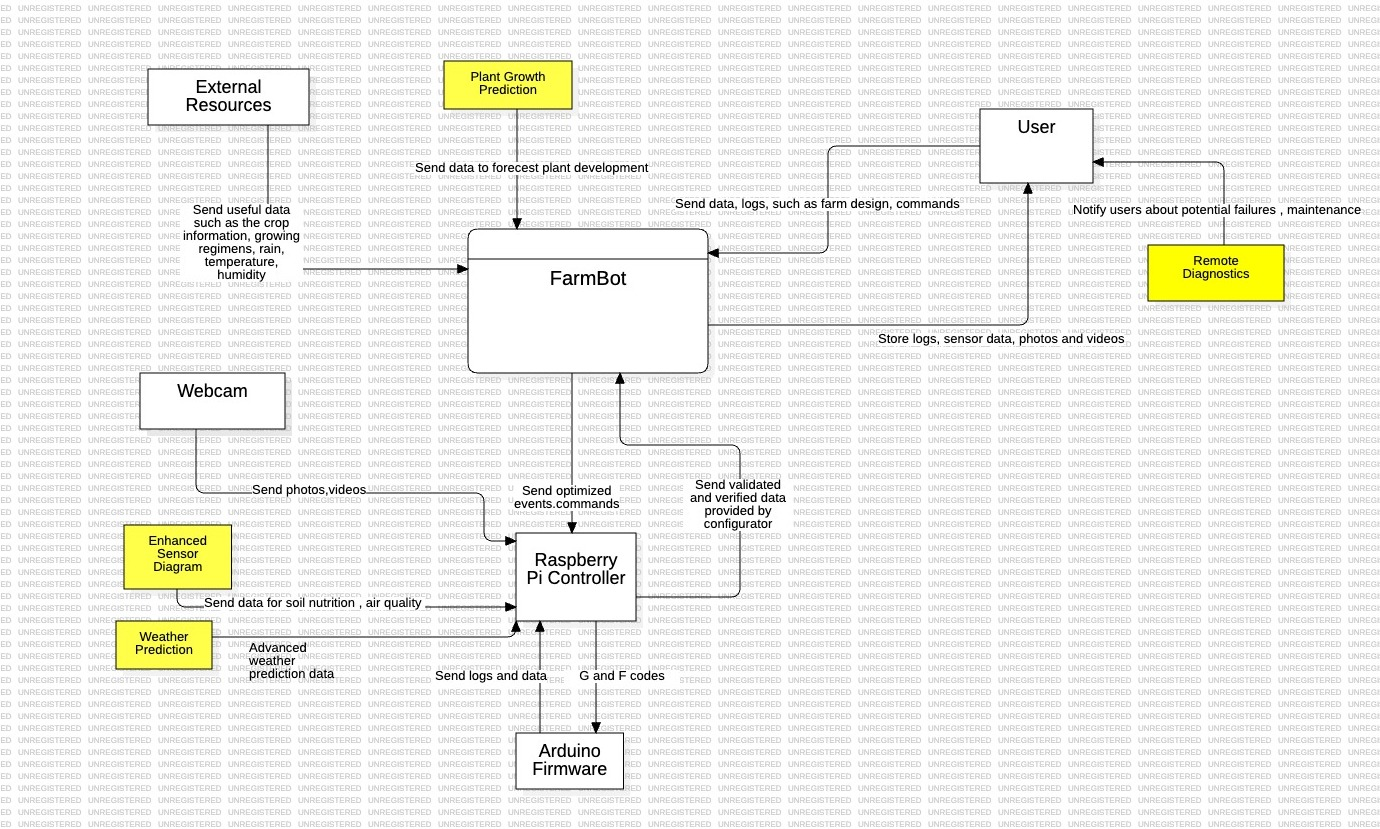
\includegraphics[scale=0.34]{./Figures/farmbot_context_diagram_suggested.jpg}
\caption{FarmBot Context Diagram with Suggestions}
\end{figure}


The system's architecture, designed to automate precision farming through FarmBot, interacts with various external and internal components. This section discusses improvements in the context of the system's interaction with its environment, highlighting four key areas for enhancement.

\subsubsection{Enhanced Sensor Integration}
\textbf{Context and Explanation:} Integrating a broader range of environmental sensors into FarmBot's system can significantly improve its adaptive capabilities. Enhanced sensors for detecting soil nutrition and air quality will allow FarmBot to respond more dynamically to the needs of the plants and the conditions of their environment. This could involve incorporating new sensor types that measure specific nutrient levels in the soil or detect pollutants in the air that could affect plant growth.

\textbf{Suggested Improvements:}
\begin{itemize}
    \item Incorporate nitrogen, phosphorus, and potassium (NPK) soil sensors to optimize fertilizer application.
    \item Add air quality sensors to monitor the presence of pollutants that could harm plant health.
    \item Develop a sensor data aggregation module in the software to analyze data from multiple sources for comprehensive environmental assessment.
\end{itemize}

\subsubsection{Advanced Weather Prediction Integration}
\textbf{Context and Explanation:} Weather plays a crucial role in farming operations. By integrating advanced weather prediction models that utilize machine learning to process historical weather data, FarmBot can proactively adjust its operations—such as watering, planting, and harvesting schedules—based on accurate weather forecasts.

\textbf{Suggested Improvements:}
\begin{itemize}
    \item Partner with advanced weather prediction services or invest in the development of proprietary weather prediction algorithms.
    \item Implement machine learning models that can analyze patterns in long-term weather data to forecast local weather conditions with higher accuracy.
    \item Automatically adjust FarmBot's operational schedules based on weather predictions to optimize plant growth and resource usage.
\end{itemize}

\subsubsection{Plant Growth Prediction Models}
\textbf{Context and Explanation:} Predicting plant growth stages and harvest times can significantly enhance the scheduling efficiency of FarmBot. Integrating plant growth prediction models that leverage historical growth data and current environmental conditions will allow for more precise planning of farming operations.

\textbf{Suggested Improvements:}
\begin{itemize}
    \item Develop or integrate existing plant growth models into FarmBot's software, tailored to the variety of plants supported by the system.
    \item Use accumulated data from FarmBot's operations and external data sources to refine and validate the growth models continuously.
    \item Provide users with predictions on growth stages and optimal harvest times, enhancing the planning and execution of farming tasks.
\end{itemize}

\subsubsection{Remote Diagnostics and Proactive Maintenance}
\textbf{Context and Explanation:} Ensuring the reliability of FarmBot's operations requires a system for early detection of potential failures or maintenance needs. Implementing a framework for remote diagnostics and proactive maintenance can help in identifying issues before they lead to system downtime.

\textbf{Suggested Improvements:}
\begin{itemize}
    \item Develop diagnostic algorithms that monitor system performance and predict potential failures based on operational data and sensor readings.
    \item Implement a maintenance scheduling module that alerts users to upcoming maintenance tasks and suggests optimal times for their completion.
    \item Allow for remote firmware updates and system checks to ensure that FarmBot operates with the latest software and within optimal performance parameters.
\end{itemize}

Each of these improvements aims to enhance the adaptability, efficiency, and reliability of the FarmBot system, leveraging advanced technologies and data-driven strategies to optimize precision farming operations.


\subsection{External Interfaces}

\begin{figure}[H]
    \centering
\includesvg[inkscapelatex=false, scale=0.42]{./Figures/external_interface_class_diagram_suggestions.svg}
\caption{Class Diagram for External Interfaces with Suggestions}
\end{figure}


This section outlines the external interfaces of the FarmBot system, highlighting the integration of both original and suggested interfaces to enhance system functionality. The context diagram (not included here) visually represents these interfaces and their connections. The following descriptions detail how suggested interfaces can complement and expand the capabilities of the existing system.

\subsubsection{Suggested External Interfaces}

\textbf{Plant Database API}
\begin{itemize}
    \item \textbf{Purpose:} To enrich FarmBot's knowledge base with extensive plant species data and their specific growth requirements, facilitating more informed decision-making for planting strategies.
    \item \textbf{Improvements:} Integration of a comprehensive plant database allows for automated, species-specific care routines, optimizing growth conditions for a diverse range of crops and enhancing yield efficiency.
\end{itemize}

\textbf{GPS Communication Interface}
\begin{itemize}
    \item \textbf{Purpose:} To provide precise geolocation capabilities for FarmBot, enabling accurate mapping of the farming area and plant locations.
    \item \textbf{Improvements:} With accurate GPS data, FarmBot can perform tasks with enhanced precision, such as targeted watering or planting, reducing resource waste and improving operational efficiency.
\end{itemize}

\textbf{Weather API}
\begin{itemize}
    \item \textbf{Purpose:} To fetch real-time and forecasted weather data, allowing FarmBot to adapt its operations based on current and upcoming weather conditions.
    \item \textbf{Improvements:} Weather adaptability ensures that FarmBot can make proactive adjustments to its routines, such as delaying watering before rain, thus optimizing resource use and protecting plants from adverse weather.
\end{itemize}

\textbf{Diagnostic and Logging API}
\begin{itemize}
    \item \textbf{Purpose:} To collect detailed diagnostics and operational logs from FarmBot, facilitating remote troubleshooting and system optimization.
    \item \textbf{Improvements:} Enhanced diagnostic capabilities enable predictive maintenance and quick resolution of issues, improving system reliability and uptime.
\end{itemize}

\subsubsection{Integration with Existing Interfaces}

The suggested interfaces complement the existing system's capabilities, forming a cohesive and intelligent farming solution:
\begin{itemize}
 

   \item  The \textbf{User Interface API} becomes a more powerful tool for users, offering access to a broader range of data and controls, from selecting plants from the \textbf{Plant Database API} to viewing weather forecasts via the \textbf{Weather API}.
   \item The \textbf{Sensor Data Interface} and \textbf{GPS Communication Interface} work in tandem to provide environmental and locational data, enhancing the precision of FarmBot's operations.
   \item  Integration of the \textbf{Diagnostic and Logging API} with the \textbf{Remote Update API} ensures that FarmBot's software remains up-to-date and operates efficiently, with maintenance and updates informed by comprehensive diagnostic data.
\end{itemize}
\subsubsection{Improvement Recommendations}

To fully leverage the potential of the suggested external interfaces, the following recommendations are proposed:

\begin{itemize}
  

  \item  Data Synchronization: Implement robust data synchronization mechanisms between the FarmBot system and the external APIs to ensure real-time accuracy and responsiveness.
  \item  User-Centric Design: Continuously refine the User Interface API to present the enriched data and controls in an intuitive and accessible manner, enhancing the user experience.
  \item  Security and Privacy: Ensure all external communications are encrypted, and data privacy is maintained, especially when integrating third-party APIs like weather services and GPS data providers.

By incorporating these suggested external interfaces and adhering to the improvement recommendations, the FarmBot system can achieve significant advancements in automation, efficiency, and user engagement.
\end{itemize}

\subsection{Interaction Scenarios}

This section includes one activity diagram to illustrate an interaction sequence that takes place over the external interfaces based on the suggested improvements. The chosen scenario represents one of the most complex interactions within the FarmBot system, showcasing how the system can be enhanced for better performance and efficiency.

\begin{figure}[H]
    \centering
    \includesvg[inkscapelatex=false, scale=0.7]{./Figures/external_interface_suggestion_weather_data_api_diagram.svg}
    \caption{External Interface Suggestion Weather Data API Activity Diagram}
\end{figure}

\subsubsection{External Interface Weather Data API Interaction}

The activity diagram illustrates the interaction between the FarmBot system and the external weather data API based on suggested improvements. This interaction is critical for enhancing the system's ability to adapt to weather conditions and optimize agricultural tasks accordingly.

\textbf{Steps in the Interaction Sequence:}
\begin{enumerate}
    \item \textbf{API Initialization:} The FarmBot system initializes a connection to the weather data API service to start the data retrieval process.
    \item \textbf{Enhanced Forecast Request:} An improved request for detailed weather forecast data is sent from the FarmBot system to the weather data API.
    \item \textbf{Advanced Data Retrieval:} The weather data API processes the request and retrieves comprehensive weather forecast data, including temperature, humidity, precipitation, and wind speed.
    \item \textbf{Data Transmission:} The detailed forecast data is transmitted back to the FarmBot system.
    \item \textbf{Enhanced Data Analysis:} The FarmBot system analyzes the received weather data using advanced algorithms to determine potential impacts on agricultural activities with higher accuracy.
    \item \textbf{Proactive Schedule Adjustment:} Based on the enhanced analysis, the system proactively adjusts the scheduling of tasks such as watering, planting, and harvesting to optimize operations in anticipation of forecasted weather conditions.
    \item \textbf{User Notification:} The system sends detailed notifications to the user about the adjusted schedules and any significant weather events that may affect the farm.
    \item \textbf{Detailed Logging:} All interactions, data points, and adjustments are logged with additional details for future analysis and reporting.
\end{enumerate}

This interaction scenario highlights the integration of enhanced weather data into the FarmBot system, showcasing the system's improved ability to proactively adjust operations based on detailed and accurate weather forecasts. The suggested improvements aim to increase the system's efficiency, reliability, and responsiveness to environmental changes, ensuring optimal agricultural management.

    

\section{Functional View}

The Functional View provides a detailed perspective on the functionalities of the enhanced FarmBot system, illustrating how various components interact to achieve the system's goals. This view is crucial for understanding the operational aspects of the system and how it meets the needs of its users.

\subsection{Stakeholders’ Uses of This View}

The Functional View is utilized by various stakeholders to comprehend the operational workflows and interactions within the enhanced FarmBot system. Key stakeholders and their uses of this view include:

\begin{itemize}
    \item \textbf{Developers:} Use this view to understand the interactions between components and to implement or modify system functionalities accordingly.
    \item \textbf{System Architects:} Leverage this view to ensure that the system’s design supports the required functionalities and interactions.
    \item \textbf{Project Managers:} Reference this view to plan and manage development tasks, ensuring that all functional requirements are met.
    \item \textbf{End Users:} Gain insights into how the system's functionalities are structured and how different components work together to provide the desired outcomes.
    \item \textbf{Quality Assurance Teams:} Use this view to design test cases that validate the functional interactions between system components.
    \item \textbf{Maintenance Teams:} Reference this view to understand the functional dependencies and to diagnose and troubleshoot issues effectively.
\end{itemize}

\subsection{Component Diagram}

This section includes a Component Diagram and its explanations for the enhanced FarmBot system. The diagram illustrates the core components and their provides/requires relationships.

\begin{figure}[H]
    \centering
    \includesvg[inkscapelatex=false, scale=0.42]{./Figures/farmbot_suggested_component_diagram.svg}
    \caption{Enhanced FarmBot Component Diagram}
\end{figure}

The component diagram includes the following components and their relationships:

\textbf{Core Components:}
\begin{itemize}
    \item \textbf{Web Application:}
    \begin{itemize}
        \item Requires services from the User Management API and Data Processing Module.
    \end{itemize}

    \item \textbf{Main Controller:}
    \begin{itemize}
        \item Provides control over the Sensor Controller, Actuator Controller, Logging Module, and Diagnostics Module.
    \end{itemize}

    \item \textbf{Sensor Controller:}
    \begin{itemize}
        \item Requires data from the Sensor API and Sensors.
        \item Provides data to the Data Processing Module.
    \end{itemize}

    \item \textbf{Actuator Controller:}
    \begin{itemize}
        \item Requires data from the Data Processing Module.
        \item Provides commands to the Actuators.
    \end{itemize}

    \item \textbf{Data Processing Module:}
    \begin{itemize}
        \item Requires data from the Database and Weather API.
        \item Provides processed data to the Main Controller.
        \item Requires services from the Enhanced Weather Prediction Module and Plant Growth Prediction Module.
    \end{itemize}

    \item \textbf{Network Communication Module:}
    \begin{itemize}
        \item Requires services from the Web Application and Mobile Application.
    \end{itemize}
    
    \item \textbf{Enhanced Weather Prediction Module:}
    \begin{itemize}
        \item Provides detailed weather forecasts to the Data Processing Module.
    \end{itemize}

    \item \textbf{Advanced Sensor Integration Module:}
    \begin{itemize}
        \item Provides data from additional sensors to the Sensor Controller.
    \end{itemize}

    \item \textbf{Remote Diagnostics Module:}
    \begin{itemize}
        \item Provides remote diagnostics capabilities to the Main Controller and Logging Module.
    \end{itemize}
    
    \item \textbf{Plant Growth Prediction Module:}
    \begin{itemize}
        \item Provides plant growth predictions to the Data Processing Module.
    \end{itemize}
\end{itemize}

\textbf{Explanations of the Core Components:}

\begin{itemize}
    \item \textbf{Web Application:} Allows users to interact with the FarmBot system through a web-based interface, requiring services from the User Management API and Data Processing Module for user authentication and data handling.

    \item \textbf{Main Controller:} Acts as the central control unit, coordinating the activities of the Sensor Controller, Actuator Controller, Logging Module, and Diagnostics Module.

    \item \textbf{Sensor Controller:} Manages data collection from various sensors through the Sensor API and Sensors, providing this data to the Data Processing Module for analysis.

    \item \textbf{Actuator Controller:} Controls the actuators based on the processed data received from the Data Processing Module, ensuring precise execution of agricultural tasks.

    \item \textbf{Data Processing Module:} Processes raw data from the Database and Weather API, providing valuable insights and data to the Main Controller for decision-making. It also requires services from the Enhanced Weather Prediction Module and Plant Growth Prediction Module to optimize agricultural tasks.

    \item \textbf{Network Communication Module:} Ensures seamless communication between the Web Application, Mobile Application, and other system components, facilitating data exchange and user interaction.
    
    \item \textbf{Enhanced Weather Prediction Module:} Provides detailed weather forecasts to the Data Processing Module, enhancing the system's ability to make informed decisions based on weather conditions.

    \item \textbf{Advanced Sensor Integration Module:} Integrates additional sensors, such as air quality sensors and nutrient sensors, into the Sensor Controller, providing more comprehensive environmental data.

    \item \textbf{Remote Diagnostics Module:} Enables remote monitoring and diagnostics of the FarmBot system, allowing for proactive maintenance and issue detection.

    \item \textbf{Plant Growth Prediction Module:} Uses historical data and advanced algorithms to predict plant growth, optimizing planting and harvesting schedules.
\end{itemize}

The enhanced component diagram and the explanations provided illustrate how the suggested improvements will integrate into the existing FarmBot system, enhancing its capabilities and performance.



\subsection{Internal Interfaces}

This section includes an Internal Interfaces Class Diagram for the suggested improvements. The following are the two suggested internal interfaces for the FarmBot project:

\begin{figure}[H]
    \centering
    \includesvg[inkscapelatex=false, scale=0.7]{./Figures/suggested_internal_interfaces.svg}
    \caption{Suggested Internal Interfaces Class Diagram}
\end{figure}

\subsubsection{Logging Interface}

The Logging Interface enhances the FarmBot system by providing robust event logging capabilities. This interface ensures that all significant events and actions are recorded for future reference and troubleshooting.

\textbf{Operations:}
\begin{itemize}
    \item \textbf{initializeLogger()}: Sets up the logging system for recording events.
    \item \textbf{logEvent(String eventDescription)}: Records a specific event with its description.
    \item \textbf{retrieveLogs(Date startDate, Date endDate)}: Retrieves logs within the specified date range.
    \item \textbf{clearLogs()}: Clears all recorded logs from the system.
\end{itemize}

\subsubsection{Diagnostic Interface}

The Diagnostic Interface is designed to maintain the health of the FarmBot system by regularly checking for potential issues and generating diagnostic reports. This interface ensures proactive maintenance and reduces system downtime.

\textbf{Operations:}
\begin{itemize}
    \item \textbf{initializeDiagnostics()}: Sets up the diagnostic system for monitoring the FarmBot.
    \item \textbf{runDiagnostics()}: Executes a diagnostic check on the system and generates a report.
    \item \textbf{scheduleDiagnostics(Date date)}: Schedules a diagnostic check for a specified date and time.
    \item \textbf{getDiagnosticHistory()}: Retrieves a history of past diagnostic reports for review.
\end{itemize}

These additional interfaces enhance the FarmBot system by providing robust logging and diagnostic capabilities. Logging ensures that all significant events and actions are recorded for future reference and troubleshooting, while diagnostics help maintain the system's health by regularly checking for potential issues and generating reports.


\subsection{Interaction Patterns}

This section includes a Sequence Diagram to show messaging sequences taking place among the system components over the internal interfaces for the suggested improvements. This diagram illustrates how different components of the enhanced FarmBot system interact through internal interfaces to perform various operations.
\begin{figure}[H]
    \centering
    \includesvg[inkscapelatex=false, scale=0.7]{./Figures/internal_interface_suggestion_logging_interface_sequence_diagram.svg}
    \caption{Internal Interface Logging Interface Sequence Diagram}
\end{figure}

\subsubsection{Logging Interface Interaction Pattern}

The Logging Interface Interaction Pattern illustrates the sequence of messages exchanged between system components when recording and managing logs. This pattern is essential for maintaining detailed records of system activities, ensuring transparency, and facilitating troubleshooting.

\textbf{Sequence of Operations:}
\begin{enumerate}
    \item \textbf{Event Occurrence:} An event occurs within the FarmBot system that needs to be logged (e.g., sensor data collection, user command execution).
    \item \textbf{Log Event:} The component where the event occurred sends a log message to the Logging Interface.
    \item \textbf{Logging Interface:} The Logging Interface receives the log message and processes it.
    \item \textbf{Log Storage:} The processed log message is stored in the logging database.
    \item \textbf{Retrieve Logs: (Optional)} When needed, components or users can request to retrieve logs from the Logging Interface.
    \item \textbf{Provide Logs:} The Logging Interface retrieves the requested logs from the logging database and provides them to the requesting component or user.
\end{enumerate}

This interaction pattern demonstrates the importance of seamless communication between system components for logging activities, highlighting the system's ability to maintain detailed records and support efficient troubleshooting.

These interaction patterns provide a comprehensive view of the messaging sequences within the enhanced FarmBot system, ensuring efficient communication between system components over the internal interfaces.



\section{Information View}

The Information View for the suggested improvements provides a detailed perspective of the enhanced data structures and information flow within the FarmBot system. It highlights how data is organized, stored, and accessed, ensuring efficient data management and utilization. This view is crucial for understanding the system's enhanced data architecture and how it supports various new functionalities.


\subsection{Stakeholders’ Uses of This View}

The Information View for the suggested improvements is utilized by various stakeholders to comprehend the enhanced data architecture and information flow within the FarmBot system. Key stakeholders and their uses of this view include:

\begin{itemize}
    \item \textbf{Database Administrators:} Use this view to understand the enhanced database schema, manage data storage, and ensure data integrity and security.
    \item \textbf{Developers:} Reference this view to design and implement new data-related features, ensuring that data handling aligns with the improved system architecture.
    \item \textbf{System Architects:} Leverage this view to ensure that the enhanced data architecture supports the system's functional and non-functional requirements.
    \item \textbf{Project Managers:} Utilize this view to understand the data dependencies and plan data-related tasks and resource allocation effectively.
    \item \textbf{End Users:} Gain insights into how their data is stored, processed, and utilized within the enhanced system, promoting transparency and trust.
    \item \textbf{Quality Assurance Teams:} Use this view to design test cases that validate the enhanced data flow and data integrity within the system.
\end{itemize}

The detailed understanding provided by the Information View ensures that data is managed efficiently, supporting the system's operational needs and user requirements.

\subsubsection{Database Class Diagram with Suggestions}

The Extended Database Class Diagram illustrates the key data objects and their interrelationships within the enhanced FarmBot system. This diagram serves as a reference for understanding how data is structured and accessed, ensuring clear and efficient data management.

\textbf{Key Data Objects:}
\begin{itemize}
    \item \textbf{Planting Data:} Holds records for plant species, planting coordinates, sowing depth, and spacing requirements.
    \item \textbf{Environmental Data:} Stores readings from environmental sensors, including moisture levels, temperature, and weather conditions.
    \item \textbf{Operation Logs:} Contains a historical record of all operations performed by FarmBot, such as watering, weeding, and fertilizing actions, along with timestamps and outcomes.
    \item \textbf{User Account Data:} Manages user information, including credentials, configuration preferences, and roles.
    \item \textbf{Scheduling Data:} Keeps track of planting and watering schedules, task prioritization, and event triggers based on environmental data.
    \item \textbf{PlantPastPerformanceVariance:} Measures the variance in past performance of plants, aiding in the prediction of future growth patterns.
    \item \textbf{PlantEnvironmentResponse:} Quantifies each plant's responsiveness to environmental conditions.
    \item \textbf{PlantGeneticData:} Contains genetic information of the plants, supporting advanced analysis for breeding optimization and genetic resilience.
    \item \textbf{KnownPests:} A record of pests known to affect the farming area.
    \item \textbf{WeatherAnomalies:} Describes historical weather anomalies in the area.
    \item \textbf{DroughtSeason:} Indicates whether the current season is prone to drought.
    \item \textbf{PreventiveMaintenance:} Outlines scheduled maintenance activities for FarmBot's machinery.
    \item \textbf{RecordingSchedule:} Specifies the schedule for recording various operational data points.
\end{itemize}

\textbf{Descriptions of Non-Obvious Names:}
\begin{itemize}
    \item \textbf{SowingDepth:} The depth at which seeds are planted to ensure optimal growth.
    \item \textbf{WeatherCondition:} A detailed description of the current weather, including factors like precipitation and wind speed.
    \item \textbf{Outcome:} The result of an operation, indicating success or failure and any relevant notes.
    \item \textbf{PlantPastPerformanceVariance:} A measure of how much a plant's past growth deviates from expected patterns.
    \item \textbf{PlantEnvironmentResponse:} A metric indicating how well a plant responds to varying environmental conditions.
    \item \textbf{PlantGeneticData:} Information about the genetic makeup of a plant, useful for understanding its traits and potential resilience.
    \item \textbf{KnownPests:} Details of pests that could potentially affect the crops, aiding in preventive measures.
    \item \textbf{WeatherAnomalies:} Historical data on unusual weather patterns to better prepare for future events.
    \item \textbf{DroughtSeason:} A boolean attribute indicating whether the current season is prone to drought conditions.
    \item \textbf{PreventiveMaintenance:} Scheduled activities aimed at preventing breakdowns of the FarmBot system.
    \item \textbf{RecordingSchedule:} Timetables for recording data points to ensure consistent data collection.
\end{itemize}

This Information View, along with the Extended Database Class Diagram, provides a comprehensive understanding of the enhanced FarmBot system's data architecture, ensuring efficient data management and utilization.


\subsection{Database Class Diagram}

\begin{figure}[H]
    \centering
    \includesvg[inkscapelatex=false, scale=0.42]{./Figures/LogicDiagramExtended.svg}
    \caption{Database Class Diagram with Suggestions}
\end{figure}

This section details the enhancements to the FarmBot system's logical database, specifically focusing on the addition of new attributes to Plant Data, Environmental Data, and Scheduling Data. These improvements aim to refine FarmBot's operational efficiency, adaptability, and data analytics capabilities.

\subsubsection{Enhancements to Plant Data}

\textbf{Plant Data} has been augmented with the following attributes to provide a more comprehensive understanding of each plant's performance and requirements:

\begin{itemize}
    \item \textbf{plantPastPerformanceVariance (Float):} Measures the variance in past performance of plants, aiding in the prediction of future growth patterns and identifying plants that deviate from expected growth trajectories.
    \item \textbf{plantEnvironmentResponse (Float):} Quantifies each plant's responsiveness to environmental conditions, enabling more personalized care strategies that adapt to the plant's specific needs.
    \item \textbf{plantGeneticData (Object):} Contains genetic information of the plants, supporting advanced analysis for breeding optimization and genetic resilience to pests or diseases.
\end{itemize}

\subsubsection{Enhancements to Environmental Data}

\textbf{Environmental Data} now includes attributes that capture broader ecological and meteorological factors:

\begin{itemize}
    \item \textbf{knownPests (Object):} A record of pests known to affect the farming area, facilitating targeted pest management strategies.
    \item \textbf{weatherAnomalies (String):} Describes historical weather anomalies in the area, providing insights for better preparation against unusual weather patterns.
    \item \textbf{droughtSeason (Boolean):} Indicates whether the current season is prone to drought, aiding in water conservation efforts and drought-resistant planting decisions.
\end{itemize}

\subsubsection{Enhancements to Scheduling Data}

\textbf{Scheduling Data} has been enhanced with attributes focused on maintenance and operational recording:

\begin{itemize}
    \item \textbf{preventiveMaintenance (Object):} Outlines scheduled maintenance activities for FarmBot's machinery, aiming to prevent equipment failure and extend the system's lifespan.
    \item \textbf{recordingSchedule (Object):} Specifies the schedule for recording various operational data points, ensuring comprehensive data collection for analysis and optimization.
\end{itemize}

\subsubsection{Class Diagram with Associations}
In the class diagram, these newly added attributes would be illustrated as part of their respective classes. Associations include:
- \textit{Plant Data} linked with \textit{Scheduling Data} to adjust care schedules based on plant genetics and environmental response.
- \textit{Environmental Data} associated with \textit{Plant Data} to correlate known pests and weather anomalies with plant health and performance.
- \textit{Scheduling Data} connected to \textit{Diagnostic and Logging API} to ensure maintenance and data recording activities are logged for future reference.

\textbf{Associations and Relationships}

- \textit{Plant Data} is linked to \textit{Environmental Data} through a relationship that allows the system to adjust planting parameters based on current environmental conditions.
- \textit{Operation Logs} are associated with both \textit{User Account Data} and \textit{Scheduling Data} to track which user initiated an operation and whether it was scheduled or triggered by an event.
- \textit{Environmental Data} interacts with \textit{Scheduling Data} to trigger specific tasks (e.g., watering) when certain environmental thresholds are met.

\textbf{Non-Obvious Names and Descriptions}

- \textit{SowingDepth}: The depth at which seeds are planted to ensure optimal growth.
- \textit{WeatherCondition}: A detailed description of the current weather, including factors like precipitation and wind speed.
- \textit{Outcome}: The result of an operation, indicating success or failure and any relevant notes.
- \textit{plantPastPerformanceVariance}: A measure of how much a plant's past growth deviates from expected patterns.
- \textit{plantEnvironmentResponse}: A metric indicating how well a plant responds to varying environmental conditions.
- \textit{plantGeneticData}: Information about the genetic makeup of a plant, useful for understanding its traits and potential resilience.
- \textit{knownPests}: Details of pests that could potentially affect the crops, aiding in preventive measures.
- \textit{weatherAnomalies}: Historical data on unusual weather patterns to better prepare for future events.
- \textit{droughtSeason}: A boolean attribute indicating whether the current season is prone to drought conditions.
- \textit{preventiveMaintenance}: Scheduled activities aimed at preventing breakdowns of the FarmBot system.
- \textit{recordingSchedule}: Timetables for recording data points to ensure consistent data collection.

\textbf{Implementation Considerations
}
Incorporating these attributes requires updating the FarmBot software to leverage this enriched data for operational decision-making. This might involve algorithm updates, user interface adjustments for data visualization, and enhanced analytics capabilities to interpret the new data types.

These database enhancements are poised to significantly improve FarmBot's precision agriculture capabilities, making the system more responsive to plant and environmental variables and proactive in maintenance scheduling. The goal is to optimize plant health, yield, and system reliability through data-driven insights.


\subsection{Operations on Data}

Descriptions of the operations are given in the extended database class diagram. These operations deal with the storage and handling of information regarding various aspects such as planting data, environmental data, operation logs, user account data, and scheduling data. The operations include typical CRUD (Create, Read, Update, Delete) operations, ensuring efficient data management.

\textbf{Operations on Data:}

\begin{itemize}
    \item \textbf{Planting Data:}
    \begin{itemize}
        \item \textbf{Create:} Add new plant species records, planting coordinates, sowing depth, and spacing requirements.
        \item \textbf{Read:} Retrieve information about specific plant species, their planting coordinates, sowing depth, and spacing requirements.
        \item \textbf{Update:} Modify existing records for plant species, planting coordinates, sowing depth, and spacing requirements.
        \item \textbf{Delete:} Remove records for plant species, planting coordinates, sowing depth, and spacing requirements.
    \end{itemize}
    
    \item \textbf{Environmental Data:}
    \begin{itemize}
        \item \textbf{Create:} Add new sensor readings for moisture levels, temperature, and weather conditions.
        \item \textbf{Read:} Retrieve sensor readings to assess current environmental conditions.
        \item \textbf{Update:} Modify existing sensor readings as needed.
        \item \textbf{Delete:} Remove outdated or incorrect sensor readings.
    \end{itemize}
    
    \item \textbf{Operation Logs:}
    \begin{itemize}
        \item \textbf{Create:} Record new operations performed by FarmBot, such as watering, weeding, and fertilizing actions, along with timestamps and outcomes.
        \item \textbf{Read:} Retrieve historical records of operations for analysis and reporting.
        \item \textbf{Update:} Update operation logs to correct any errors or add additional details.
        \item \textbf{Delete:} Delete old operation logs that are no longer needed.
    \end{itemize}
    
    \item \textbf{User Account Data:}
    \begin{itemize}
        \item \textbf{Create:} Add new user accounts, including credentials, configuration preferences, and roles.
        \item \textbf{Read:} Retrieve user account information for authentication and personalization.
        \item \textbf{Update:} Modify existing user account information, such as updating passwords or preferences.
        \item \textbf{Delete:} Remove user accounts that are no longer active.
    \end{itemize}
    
    \item \textbf{Scheduling Data:}
    \begin{itemize}
        \item \textbf{Create:} Create new schedules for planting, watering, task prioritization, and event triggers based on environmental data.
        \item \textbf{Read:} Retrieve existing schedules to determine upcoming tasks and events.
        \item \textbf{Update:} Update schedules to reflect changes in task priorities or environmental conditions.
        \item \textbf{Delete:} Delete outdated or incorrect schedules.
    \end{itemize}

    \item \textbf{PlantPastPerformanceVariance:}
    \begin{itemize}
        \item \textbf{Create:} Record variance data for new plants.
        \item \textbf{Read:} Retrieve variance data for analysis.
        \item \textbf{Update:} Update variance data based on new growth information.
        \item \textbf{Delete:} Remove outdated variance data.
    \end{itemize}

    \item \textbf{PlantEnvironmentResponse:}
    \begin{itemize}
        \item \textbf{Create:} Add new data on plant responses to environmental conditions.
        \item \textbf{Read:} Retrieve response data for specific plants.
        \item \textbf{Update:} Modify response data as new information is gathered.
        \item \textbf{Delete:} Delete old response data that is no longer relevant.
    \end{itemize}

    \item \textbf{PlantGeneticData:}
    \begin{itemize}
        \item \textbf{Create:} Record genetic information for new plants.
        \item \textbf{Read:} Retrieve genetic data for analysis.
        \item \textbf{Update:} Update genetic data with new findings.
        \item \textbf{Delete:} Remove genetic data that is outdated or no longer needed.
    \end{itemize}

    \item \textbf{KnownPests:}
    \begin{itemize}
        \item \textbf{Create:} Add records of pests known to affect the farming area.
        \item \textbf{Read:} Retrieve information about known pests.
        \item \textbf{Update:} Update pest records with new findings.
        \item \textbf{Delete:} Delete pest records that are no longer relevant.
    \end{itemize}

    \item \textbf{WeatherAnomalies:}
    \begin{itemize}
        \item \textbf{Create:} Record historical weather anomalies.
        \item \textbf{Read:} Retrieve data on past weather anomalies.
        \item \textbf{Update:} Update records with new weather anomaly data.
        \item \textbf{Delete:} Remove outdated weather anomaly records.
    \end{itemize}

    \item \textbf{DroughtSeason:}
    \begin{itemize}
        \item \textbf{Create:} Record data on drought-prone seasons.
        \item \textbf{Read:} Retrieve information about current and past drought seasons.
        \item \textbf{Update:} Update drought season records with new data.
        \item \textbf{Delete:} Remove outdated drought season records.
    \end{itemize}

    \item \textbf{PreventiveMaintenance:}
    \begin{itemize}
        \item \textbf{Create:} Schedule new preventive maintenance activities.
        \item \textbf{Read:} Retrieve scheduled maintenance activities.
        \item \textbf{Update:} Update maintenance schedules as needed.
        \item \textbf{Delete:} Remove completed or outdated maintenance activities.
    \end{itemize}

    \item \textbf{RecordingSchedule:}
    \begin{itemize}
        \item \textbf{Create:} Set new schedules for data recording.
        \item \textbf{Read:} Retrieve existing recording schedules.
        \item \textbf{Update:} Modify recording schedules based on new requirements.
        \item \textbf{Delete:} Delete old recording schedules that are no longer needed.
    \end{itemize}
\end{itemize}

These operations ensure that the enhanced FarmBot system can efficiently manage and utilize data, supporting its various new functionalities and improving overall system performance.




\section{Deployment View}

The Deployment View provides a detailed perspective on how the enhanced FarmBot system's components are distributed across different nodes in the network. This view is crucial for understanding the physical arrangement of the system, how components communicate, and where each component is deployed. It ensures that the system's deployment aligns with its operational requirements and constraints.

\subsection{Stakeholders’ Uses of This View}

The Deployment View is utilized by various stakeholders to understand how the enhanced FarmBot system's components are distributed across different nodes in the network. Key stakeholders and their uses of this view include:

\begin{itemize}
    \item \textbf{System Administrators:} Use this view to manage and monitor the deployment of the enhanced FarmBot system, ensuring that all components are correctly deployed and communicating effectively.
    \item \textbf{Developers:} Reference this view to understand the deployment environment, aiding in the development and troubleshooting of the system.
    \item \textbf{Project Managers:} Utilize this view to plan and coordinate the deployment of system components, ensuring that deployment aligns with project timelines and objectives.
    \item \textbf{End Users:} Gain insights into how the enhanced system is deployed, providing transparency into the system's architecture and operations.
\end{itemize}

\subsection{Deployment Diagram}

This section includes an enhanced Deployment Diagram and explanations for the suggested improvements.

\begin{figure}[H]
    \centering
    \includesvg[inkscapelatex=false, scale=0.33]{./Figures/suggested_deployment_diagram.svg}
    \caption{Enhanced FarmBot Deployment Diagram with Suggestions}
\end{figure}

\subsubsection{Deployment Diagram Explanations}

The enhanced deployment diagram includes the following nodes and their connections:

\textbf{User Devices:}
\begin{itemize}
    \item \textbf{Web Browser:} Connects to the Web Server to provide a web-based interface for users.
    \item \textbf{Mobile Device:} Connects to the \textbf{mobile app} to provide a mobile interface for users.
\end{itemize}

\textbf{FarmBot Local Network:}
\begin{itemize}
    \item \textbf{FarmBot Controller:} Connects to Sensors and Actuators within the local network to manage farming tasks. It also connects to the Application Server for data processing and receiving commands.
    \item \textbf{Sensors:} Provide environmental data to the FarmBot Controller.
    \item \textbf{Actuators:} Execute farming tasks based on commands from the FarmBot Controller.
    \item \textbf{Advanced Sensor Integration Module:} Provides data from additional sensors to the FarmBot Controller.
\end{itemize}

\textbf{Cloud Services:}
\begin{itemize}
    \item \textbf{Web Server:} Hosts the web application and connects to the Application Server.
    \item \textbf{Application Server:} Processes data and commands, connects to the Database Server for data storage, and connects to the Weather API for weather data.
    \item \textbf{Database Server:} Stores data collected and processed by the FarmBot system.
    \item \textbf{Weather API:} Provides weather data to the Application Server for informed decision-making.
    \item \textbf{Enhanced Weather Prediction Module:} Provides detailed weather forecasts to the Application Server.
    \item \textbf{Remote Diagnostics Module:} Enables remote monitoring and diagnostics for the FarmBot Controller and Logging Module.
    \item \textbf{Plant Growth Prediction Module:} Provides plant growth predictions to the Application Server.
\end{itemize}

The enhanced deployment diagram and explanations illustrate how the suggested improvements will be deployed across different nodes, ensuring efficient and effective operation.

\section{Design Rationale}

\textbf{Design Rationale:} The enhanced deployment view ensures that system components are correctly distributed across different nodes, supporting efficient data processing, communication, and operational management. This view is critical for maintaining the reliability and performance of the enhanced FarmBot system.


